% Step and impulse response of an I-Glied (G(s) = K_I / s)
% Left:  step response  h(t) = K_I * t (ramp)
% Right: impulse response g(t) = K_I * sigma(t) (step)

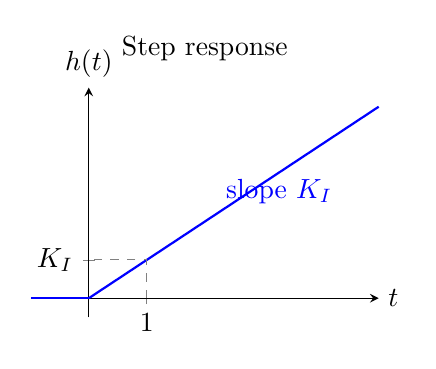
\begin{tikzpicture}
    \begin{axis}[
        width=6cm, height=4.5cm,
        xlabel={$t$}, ylabel={$h(t)$},
        title={Step response},
        axis lines=middle,
        xmin=-1, xmax=5,
        ymin=-0.5, ymax=5.5,
        xtick={1}, xticklabels={$1$},
        ytick={1}, yticklabels={$K_I$},
        every axis y label/.style={at={(ticklabel* cs:1.0)}, anchor=south},
        every axis x label/.style={at={(ticklabel* cs:1.0)}, anchor=west},
        clip=false
    ]
        \addplot[blue, thick, domain=-1:0, samples=2] {0};
        \addplot[blue, thick, domain=0:5, samples=2] {\x};
        \draw[dashed, gray] (axis cs:1,0) -- (axis cs:1,1) -- (axis cs:0,1);
        \node[blue, anchor=south west] at (axis cs:2.2,2.2) {slope $K_I$};
    \end{axis}
\end{tikzpicture}%
\hspace{0.6cm}%
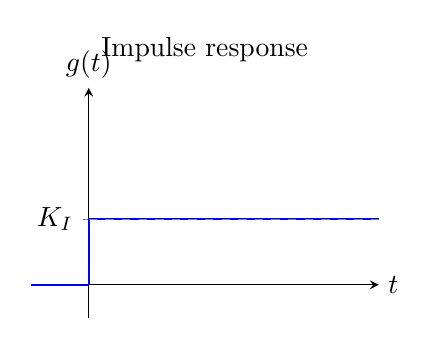
\begin{tikzpicture}
    \begin{axis}[
        width=6cm, height=4.5cm,
        xlabel={$t$}, ylabel={$g(t)$},
        title={Impulse response},
        axis lines=middle,
        xmin=-1, xmax=5,
        ymin=-0.5, ymax=3,
        xtick=\empty, ytick={1},
        yticklabels={$K_I$},
        every axis y label/.style={at={(ticklabel* cs:1.0)}, anchor=south},
        every axis x label/.style={at={(ticklabel* cs:1.0)}, anchor=west},
        clip=false
    ]
        \addplot[blue, thick, domain=-1:0, samples=2] {0};
        \addplot[blue, thick, domain=0:5, samples=2] {1};
        \draw[blue, thick] (axis cs:0,0) -- (axis cs:0,1);
        \draw[dashed, gray] (axis cs:0,1) -- (axis cs:5,1);
    \end{axis}
\end{tikzpicture}
